\begin{enumerate}
\item The maximum clock frequency in MHz of a 4-stage ripple counter, utilizing flip-flops, with each flip-flop having a propagation delay of 20 ns, is \rule{1cm}{0.10mm}. (round off to one decimal place)
\label{gate-ee-2022-29}
\hfill (GATE EE 2022)

\item The digital circuit shown \rule{1cm}{0.15mm}
\begin{center}
\begin{tikzpicture}
\ctikzset{                                   
logic ports=ieee,                   
logic ports/scale=0.5               
}                                    
\draw(-1.3,-0.56)node[nor port,anchor=out](x) {};  
%Drawing flip-flops
\draw (-1.3,-1.3) rectangle (0,0);
\draw(-1,-0.6) node{$D$};
\draw(-2,-1.1) node{$D_0$};
\draw(-0.2,-0.6) node{$Q$};
\draw(0.7,-1.3) rectangle (2,0);
\draw(1,-0.6) node{$D$};
\draw(1.8,-0.6) node{$Q$};
\draw(2.7,-1.3) rectangle (4,0);
\draw(3,-0.6) node{$D$};
\draw(3.8,-0.6) node{$Q$};
%connecting them
\draw(0,-0.6) -- (0.7,-0.6);
\draw(2,-0.6) -- (2.7,-0.6);
\draw(4,-0.6) -- (4.35,-0.6);
%drawing clk
\draw(-1.5,-2) node[above]{$CLK$} -- (3.35,-2);
%connecting clk 
\draw(-0.65,-2) -- (-0.65,-1.3);
\draw(1.35,-2) -- (1.35,-1.3);
\draw(3.35,-2) -- (3.35,-1.3);
\draw(3.35,-2) -- (4,-2);
%drawing clk edges
\draw(-0.5,-1.3) -- (-0.65,-1.1) -- (-0.8,-1.3);
\draw(1.2,-1.3) -- (1.35,-1.1) -- (1.5,-1.3);
\draw(3.2,-1.3) -- (3.35,-1.1) -- (3.5,-1.3);
%drawing Q2,Q1,Q0
%\draw(0.35,-0.6) --(0.35,0.2);
\draw(2.35,-0.6) --(2.35,0.3);
\draw(4.35,-0.6) --(4.35,0.9);
\draw(4.35,0.9) -- (-3,0.9);
\draw(2.35,0.3) -- (-2.5,0.3);
\draw(x.in 2) -|(-3,-0.7)to[short](-3,0.9);
\draw(x.in 1) -|(-2.5,-0.3)to[short](-2.5,0.3);
\draw(0.35,-0.3)node{$Q0$};
\draw(2.35,-0.35)node{$Q1$};
\draw(4.6,-0.35)node{$Q2$};
\end{tikzpicture}
\end{center}
\begin{enumerate}[label=(\Alph*)]
    \item is a divide-by-5 counter
    \item is a divide-by-7 counter
    \item is a divide-by-8 counter
    \item does not function as a counter due to disjoint cycles of states 
\end{enumerate}
\hfill{GATE IN 2022}
\item The propogation delay of the exclusive-OR(XOR) gate in the circuit in the figure is 3ns.The propogation delay of all the flip-flops is assumed to be zero.The clock(Clk) frequency provided to the circuit is 500MHz.
\label{prob:gate-ec-46.2021}
\hfill (GATE EC 2021)

\begin{tikzpicture}
\ctikzset{                                   
logic ports=ieee,                   
logic ports/scale=0.5               
}                                    
\draw(-1.3,-0.56)node[xor port,anchor=out](x) {};  
%Drawing flip-flops
\draw (-1.3,-1.3) rectangle (0,0);
\draw(-1,-0.6) node{$D2$};
\draw(0.7,-1.3) rectangle (2,0);
\draw(1,-0.6) node{$D1$};
\draw(2.7,-1.3) rectangle (4,0);
\draw(3,-0.6) node{$D0$};
%connecting them
\draw(0,-0.6) -- (0.7,-0.6);
\draw(2,-0.6) -- (2.7,-0.6);
\draw(4,-0.6) -- (4.35,-0.6);
%drawing clk
\draw(-1.5,-2) node[above]{$clk$} -- (3.35,-2);
%connecting clk 
\draw(-0.65,-2) -- (-0.65,-1.3);
\draw(1.35,-2) -- (1.35,-1.3);
\draw(3.35,-2) -- (3.35,-1.3);
%drawing clk edges
\draw(-0.5,-1.3) -- (-0.65,-1.1) -- (-0.8,-1.3);
\draw(1.2,-1.3) -- (1.35,-1.1) -- (1.5,-1.3);
\draw(3.2,-1.3) -- (3.35,-1.1) -- (3.5,-1.3);
%drawing Q2,Q1,Q0
\draw(0.35,-0.6) --(0.35,0.3);
\draw(2.35,-0.6) --(2.35,0.35);
\draw(4.35,-0.6) --(4.35,0.9);
\draw(4.35,0.9) -- (-3,0.9);
\draw(0.35,0.3) -- (-2.5,0.3);
\draw(x.in 2) -|(-3,-0.7)to[short](-3,0.9);
\draw(x.in 1) -|(-2.5,-0.3)to[short](-2.5,0.3);
\draw(0.35,0.5)node{$Q2$};
\draw(2.35,0.45)node{$Q1$};
\draw(4.35,1)node{$Q0$};
\end{tikzpicture}

Starting from the initial value of the flip-flop outputs $Q2Q1Q0 =111$ with $D2=1$,the minimum number of triggering clock edges after which the flip-flop outputs $Q2Q1Q0$ becomes 1 0 0\emph{(in integer)} is \line(1,0){12.5} 

\item  
\label{prob:gate IN 17}
For the $3$-bit binary counter shown in the figure, the output increments at every positive 
transition in the clock (CLK). Assume ideal diodes and the starting state of the counter as 
$000$. If output high is $1 V$ and output low is $0 V$, the current $I$(in mA) flowing through the 
$50 \Omega$ resistor during the $5$th clock cycle is (up to one decimal place)
\hfill(GATE IN 2018)
\begin{figure}[H]
\centering
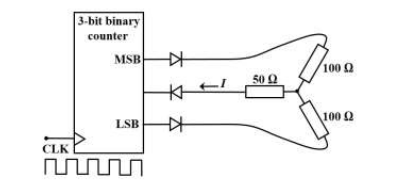
\includegraphics[width=\columnwidth]{ide/7474/figs/pic.png}
\caption{circuit}
\label{fig:lcd}
\end{figure}
\end{enumerate}
